%% LyX 1.5.3 created this file.  For more info, see http://www.lyx.org/.
%% Do not edit unless you really know what you are doing.
\documentclass[english,british]{article}
\usepackage[T1]{fontenc}
\usepackage[latin9]{inputenc}
\usepackage{url}
\usepackage{graphicx}

\makeatletter

%%%%%%%%%%%%%%%%%%%%%%%%%%%%%% LyX specific LaTeX commands.
%% Bold symbol macro for standard LaTeX users
\providecommand{\boldsymbol}[1]{\mbox{\boldmath $#1$}}


%%%%%%%%%%%%%%%%%%%%%%%%%%%%%% Textclass specific LaTeX commands.
\newenvironment{lyxcode}
{\begin{list}{}{
\setlength{\rightmargin}{\leftmargin}
\setlength{\listparindent}{0pt}% needed for AMS classes
\raggedright
\setlength{\itemsep}{0pt}
\setlength{\parsep}{0pt}
\normalfont\ttfamily}%
 \item[]}
{\end{list}}

\usepackage{babel}
\makeatother

\begin{document}

\section{Introduction to Minion}

Minion is a solver for constraint satisfaction problems. First we
introduce constraints, then give a general overview of Minion. Following
this we give instructions for installation and basic use.


\subsection{What are constraints?}

Constraints are a powerful and natural means of knowledge representation
and inference in many areas of industry and academia. Consider, for
example, the production of a university timetable. This problem's
constraints include: the maths lecture theatre has a capacity of 100
students; art history lectures require a venue with a slide projector;
no student can attend two lectures simultaneously. Constraint solving
of a combinatorial problem proceeds in two phases. First, the problem
is \emph{modelled} as a set of \emph{decision variables}, and a set
of \emph{constraints} on those variables that a solution must satisfy.
A decision variable represents a choice that must be made in order
to solve the problem. The \emph{domain} of potential values associated
with each decision variable corresponds to the options for that choice.
In our example one might have two decision variables per lecture,
representing the time and the venue. For each class of students, the
time variables of the lectures they attend may have an AllDifferent
constraint on them to ensure that the class is not timetabled to be
in two places at once. The second phase consists of using a constraint
solver to search for \emph{solutions}: assignments of values to decision
variables satisfying all constraints. The simplicity and generality
of this approach is fundamental to the successful application of constraint
solving to a wide variety of disciplines such as scheduling, industrial
design and combinatorial mathematics \cite{wallace:Survey}.

\selectlanguage{english}%
To illustrate, figure \ref{fig:Alphametic-problem} shows a simple
puzzle, where two six-digit numbers (DONALD and GERALD) are added
together to form another six-digit number (ROBERT). Each letter A,
B, D, E, G, L, N, O, R and T represents a distinct digit $0\ldots9$.
The puzzle can be represented with the expressions below, given by
Bessi\`ere and R\'egin \cite{bessiere-gac-schema}.

\begin{eqnarray*}
100000\times\textrm{D}+10000\times\textrm{O}+1000\times\textrm{N}+100\times\textrm{A}+10\times\textrm{L}+\textrm{D}\\
+100000\times\textrm{G}+10000\times\textrm{E}+1000\times\textrm{R}+100\times\textrm{A}+10\times\textrm{L}+\textrm{D}\\
=100000\times\textrm{R}+10000\times\textrm{O}+1000\times\textrm{B}+100\times\textrm{E}+10\times\textrm{R}+\textrm{T}\\
\textrm{and allDifferent}(\textrm{A, B, D, E, G, L, N, O, R, T})\end{eqnarray*}


This representation of the puzzle illustrates the main concepts of
constraint programming. A, B, D, E, G, L, N, O, R and T are variables,
each with initial domain $0\ldots9$. There are two constraints, one
representing the sum and the other representing that the variables
each take a different value. A solution is a function mapping each
variable to a value in its initial domain, such that all constraints
are satisfied. The solution to this puzzle is A=4, B=3, D=5, E=9,
G=1, L=8, N=6, O=2, R=7, T=0.

%
\begin{figure}
\begin{centering}

\includegraphics[scale=0.5]{litreview-example-alphametic}
\par\end{centering}

\caption{\label{fig:Alphametic-problem}Alphametic problem}

\end{figure}


Constraints are \emph{declarative} --- the statement of the problem
and the algorithms used to solve it are separated. This is an attractive
feature of constraints, since it can reduce the human effort required
to solve a problem. Various general purpose and specialized algorithms
exist for solving systems of constraints. A great variety of problems
can be expressed with constraints. The following list of subject areas
was taken from CSPLib \cite{csplib}:

\begin{itemize}
\item Scheduling (e.g. job shop scheduling \cite{martin-jobshop-96new}),
\item Design, configuration and diagnosis (e.g. template design \cite{proll-smith-templatedesign}),
\item Bin packing and partitioning (e.g. social golfer problem \cite{harvey01symmetry}),
\item Frequency assignment (e.g. the golomb ruler problem \cite{smith99golomb}),
\item Combinatorial mathematics (e.g. balanced incomplete block design \cite{frisch-symmetry-implied-04}),
\item Games and puzzles (e.g. maximum density still life \cite{smith-model-life}), 
\item Bioinformatics (e.g. discovering protein shapes \cite{protein-structure-problems}).
\end{itemize}
\selectlanguage{british}%

\subsection{Solving constraint problems}

\selectlanguage{english}%
The classical constraint satisfaction problem (CSP) has a finite set
of variables, each with a finite domain, and a set of constraints
over those variables. A solution to an instance of CSP is an assignment
to each variable, such that all constraints are simultaneously \emph{satisfied}
--- that is, they are all true under the assignment. Solvers typically
find one or all solutions, or prove there are no solutions. The decision
problem (`does there exist a solution?') is NP-complete \cite{apt-constraint-programming},
therefore there is no known polynomial-time procedure to find a solution.

The most common technique (and the one used by Minion) is to interleave
splitting (also called branching) and propagation. Splitting is the
basic operation of search, and propagation simplifies the CSP instance.
Apt views the solution process as the repeated transformation of the
CSP until a solution state is reached \cite{apt-constraint-programming}.
In this view, both splitting and propagation are transformations,
where propagation simplifies the CSP by removing values which cannot
take part in any solution. A splitting operation transforms a CSP
instance into two or more simpler CSP instances, and by recursive
application of splitting any CSP can be solved. 

\selectlanguage{british}%
Since splitting is an exponential-time solution method, it is important
that splitting is minimized by effective propagation. Much effort
has gone into developing propagation algorithms which are fast and
effective in removing values. Most propagation algorithms are specialized
to particular types of constraint (e.g. a vector of variables take
distinct values in any solution, the AllDifferent constraint). They
typically run in polynomial time.

\selectlanguage{english}%
Figure \ref{fig:solver-overview} is a simple representation of how
many constraint solvers (including Minion) work. The search element
is typically depth-first chronological backtracking by default, although
a solver will often allow different search algorithms to be programmed.
When searching, a variable and value must be selected. This can be
done statically or with a dynamic heuristic. The simplify component
contains a queue of constraints which need to be propagated. When
a constraint is propagated, and removes values from the variable domains,
the domain events cause other constraints to be added to the queue.
Propagation of constraints on the queue is iterated until the queue
is empty.

%
\begin{figure}
\begin{centering}
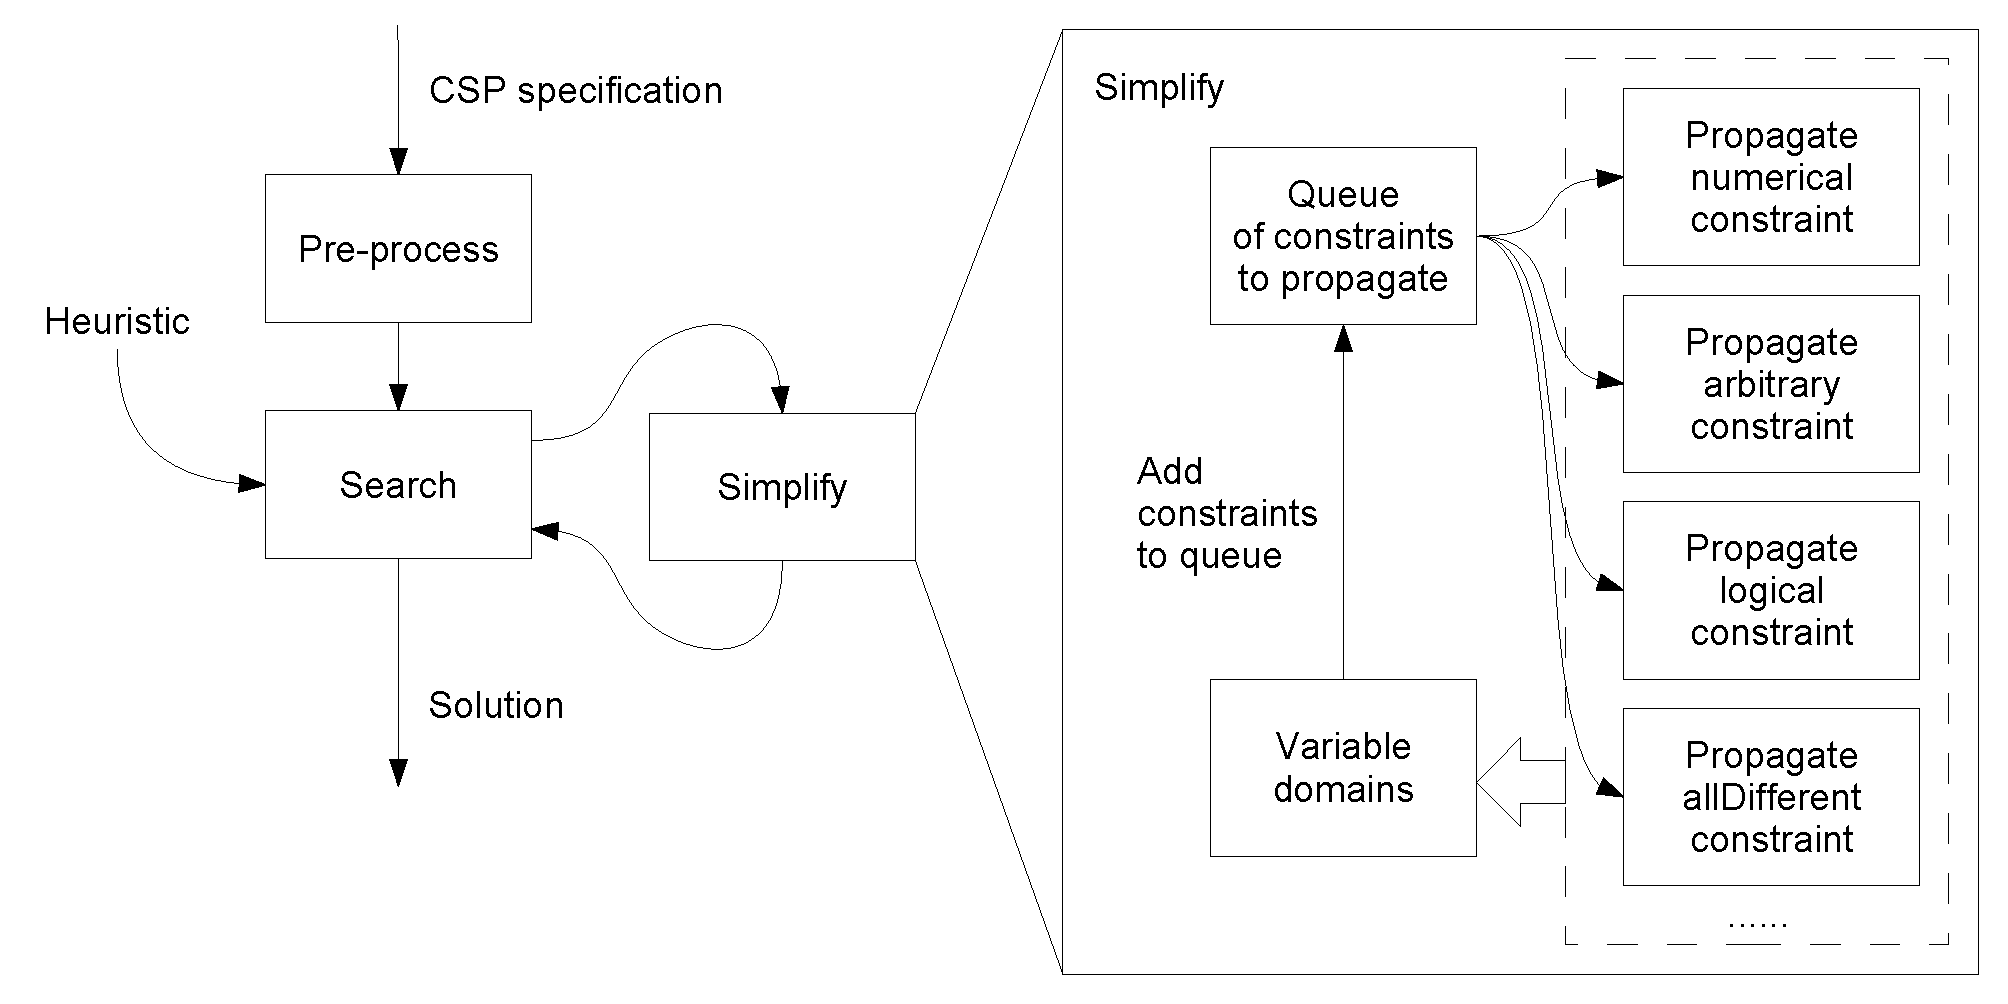
\includegraphics[width=1\textwidth]{litreview-solver-diagram}
\par\end{centering}

\caption{\label{fig:solver-overview}Overview of a constraint solver}

\end{figure}


\selectlanguage{british}%

\subsection{Minion}

Minion accepts a file describing an instance of CSP, and solves it
as described above. From the user's point of view, the most important
features are the set of constraints Minion can reason with, and the
types of variables which are supported. These are described later
in this document. This section deals with installing Minion and getting
started with it.


\subsubsection{Installing Minion}

The main Minion website is \url{http://minion.sourceforge.net/},
and this contains links to the download page. Executables are provided
for three platforms: Windows, Mac and Linux.


\subsubsection*{Installation instructions for Windows}

Download the windows archive minion-x.y.z-windows.zip and unpack,
you should find Minion executables minion.exe and minion-debug.exe
along with the required library cygwin1.dll. The executables should
work from the windows command shell cmd.exe.


\subsubsection*{Installation instructions for Mac}

Download the Mac archive minion-x.y.z-mac.zip and unpack. The contents
include universal binaries `minion' and `minion-debug' which should
work on any OS X Mac.


\subsubsection*{Installation instructions for Linux-x86 or x64}

Download the Linux archive minion-x.y.z-linux.zip and unpack. It contains
the binaries `minion' and `minion-debug'. If these binaries do not
work on your Linux distribution due to a library linking error, use
the package minion-x.y.z-linux-static.zip instead.


\subsubsection*{Compilation instructions}

If there is no executable which works on your computer, you can use
the source package (named minion-x.y.z-source.zip). To compile on
Mac and Linux, go to the source directory and issue the following
commands:

\begin{lyxcode}
./configure.sh

make~minion
\end{lyxcode}
If you have 2GB of RAM and a dual-core processor, you may prefer to
use \texttt{make minion -j2} instead. To build minion-debug, append
\texttt{DEBUG=1} to the \texttt{make} command. Executables will be
created in the \texttt{bin} subdirectory.


\subsubsection*{Trying out the executable}

On all platforms, Minion needs to be run from a command shell so that
the output can be seen. If you go to the Minion directory in a shell
and run the executable, it should output version information and a
help message. 


\subsubsection*{The debug variant}

One would normally use the non-debug variant of minion, which runs
at full speed. However, if some unexpected behaviour is observed,
running the debug variant may be helpful. It contains a large number
of assertions and other checks, and may bring to light a problem with
the input or an internal bug.


\subsubsection{Minion online help}

To see the root page of the help system, run Minion with \texttt{help}
as the only argument. The help system is hierarchical, with the following
top-level categories: constraints, input, switches and variables,
with contents as follows:

\begin{description}
\item [{\texttt{constraints}}] This category contains a description of
every constraint which is allowed in the input CSP.
\item [{\texttt{input}}] Information about the input file format.
\item [{\texttt{switches}}] Information about command-line switches.
\item [{\texttt{variables}}] A description of each type of CSP variable
supported in Minion.
\end{description}
To access the help for the alldiff constraint, for example, the command
would be \texttt{minion help constraints alldiff}. 


\subsubsection{Basic Minion use}

As a simple example of Minion input, we modelled the alphametic puzzle
in figure \ref{fig:Alphametic-problem}. The Minion input file shown
below consists of two sections: the variables, in which the 10 CSP
variables are declared along with their initial domains; and the constraints.
The allDifferent constraint in the example above is mapped into gacalldiff
here. The numerical constraint is translated into two constraints
as follows: $x+y=z$ is mapped to $x+y-z\le0$ and $x+y-z\ge0$ and
these two are represented using weightedsumleq and weightedsumgeq
respectively. The coefficients are specified first, with the coefficients
of ROBERT negated, followed by the list of variables.

\begin{lyxcode}
MINION~3~

{*}{*}VARIABLES{*}{*}~

DISCRETE~a~\{0..9\}~

DISCRETE~b~\{0..9\}~

DISCRETE~d~\{0..9\}~

DISCRETE~e~\{0..9\}~

DISCRETE~g~\{0..9\}~

DISCRETE~l~\{0..9\}~

DISCRETE~n~\{0..9\}~

DISCRETE~o~\{0..9\}~

DISCRETE~r~\{0..9\}~

DISCRETE~t~\{0..9\}~

{*}{*}CONSTRAINTS{*}{*}~

gacalldiff({[}a,b,d,e,g,l,n,o,r,t])~

weightedsumleq({[}100000,10000,1000,100,10,1,

100000,10000,1000,100,10,1,

-100000,-10000,-1000,-100,-10,-1],~

{[}d,o,n,a,l,d,g,e,r,a,l,d,r,o,b,e,r,t],0)

weightedsumgeq({[}100000,10000,1000,100,10,1,

100000,10000,1000,100,10,1,

-100000,-10000,-1000,-100,-10,-1],~

{[}d,o,n,a,l,d,g,e,r,a,l,d,r,o,b,e,r,t],0)~

{*}{*}EOF{*}{*}~
\end{lyxcode}
This example is in the Minion distribution, in directory benchmarks/small.
Executing \texttt{minion benchmarks/small/donaldgeraldrobert.minion}
gives the solution \foreignlanguage{english}{A=4, B=3, D=5, E=9, G=1,
L=8, N=6, O=2, R=7, T=0. }

\begin{lyxcode}

\end{lyxcode}
\bibliographystyle{plain}
\bibliography{/home/pn/general}

\end{document}
